\chapter{Anhang}
\section{Abbildungen}
\subsection{Zeeman-Effekt}
\begin{figure}[!ht]
    \subcaptionbox{Aufnahmen der Aufspaltung ohne äußeres Magnetfeld}{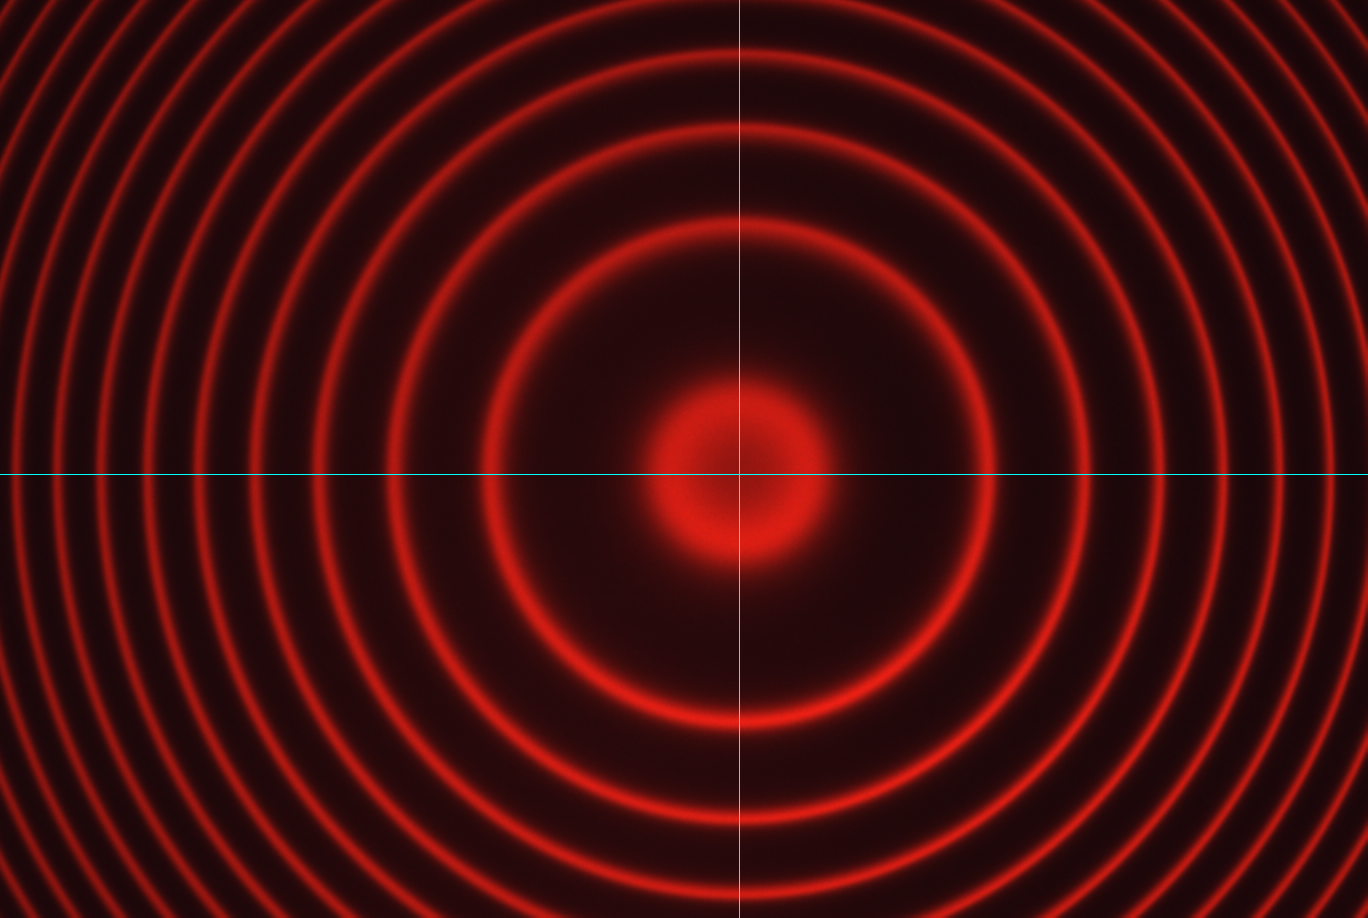
\includegraphics[width=.5\textwidth]{images/ZeemanFoto_001.png}}
    \subcaptionbox{Aufnahmen der Aufspaltung mit äußerem Magnetfeld}{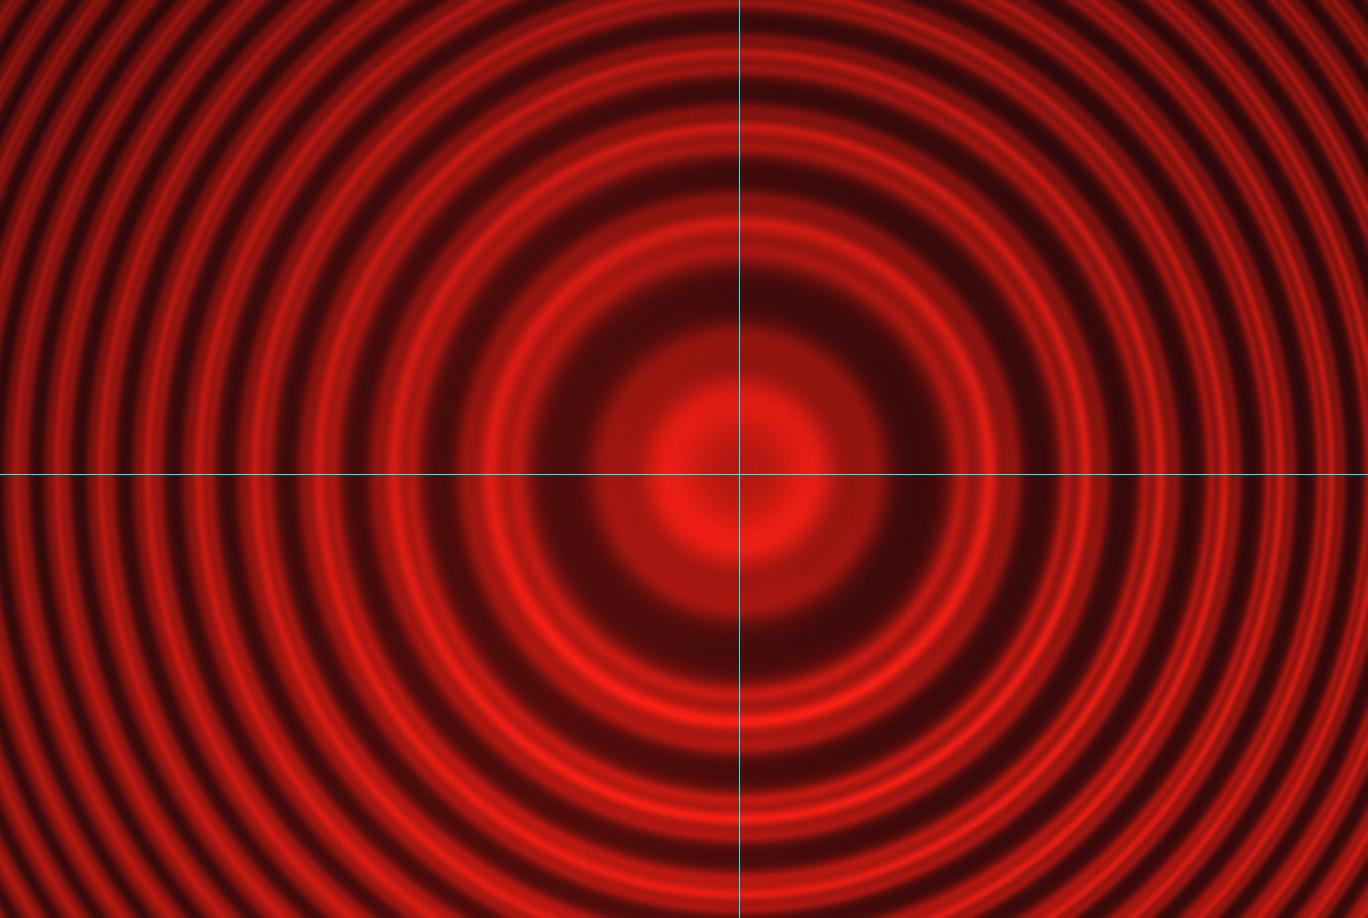
\includegraphics[width=.5\textwidth]{images/ZeemanFoto_002.png}}
    \subcaptionbox{Aufnahmen der Aufspaltung mit äußerem Magnetfeld ($\sigma^{\pm}$-Komponente)}{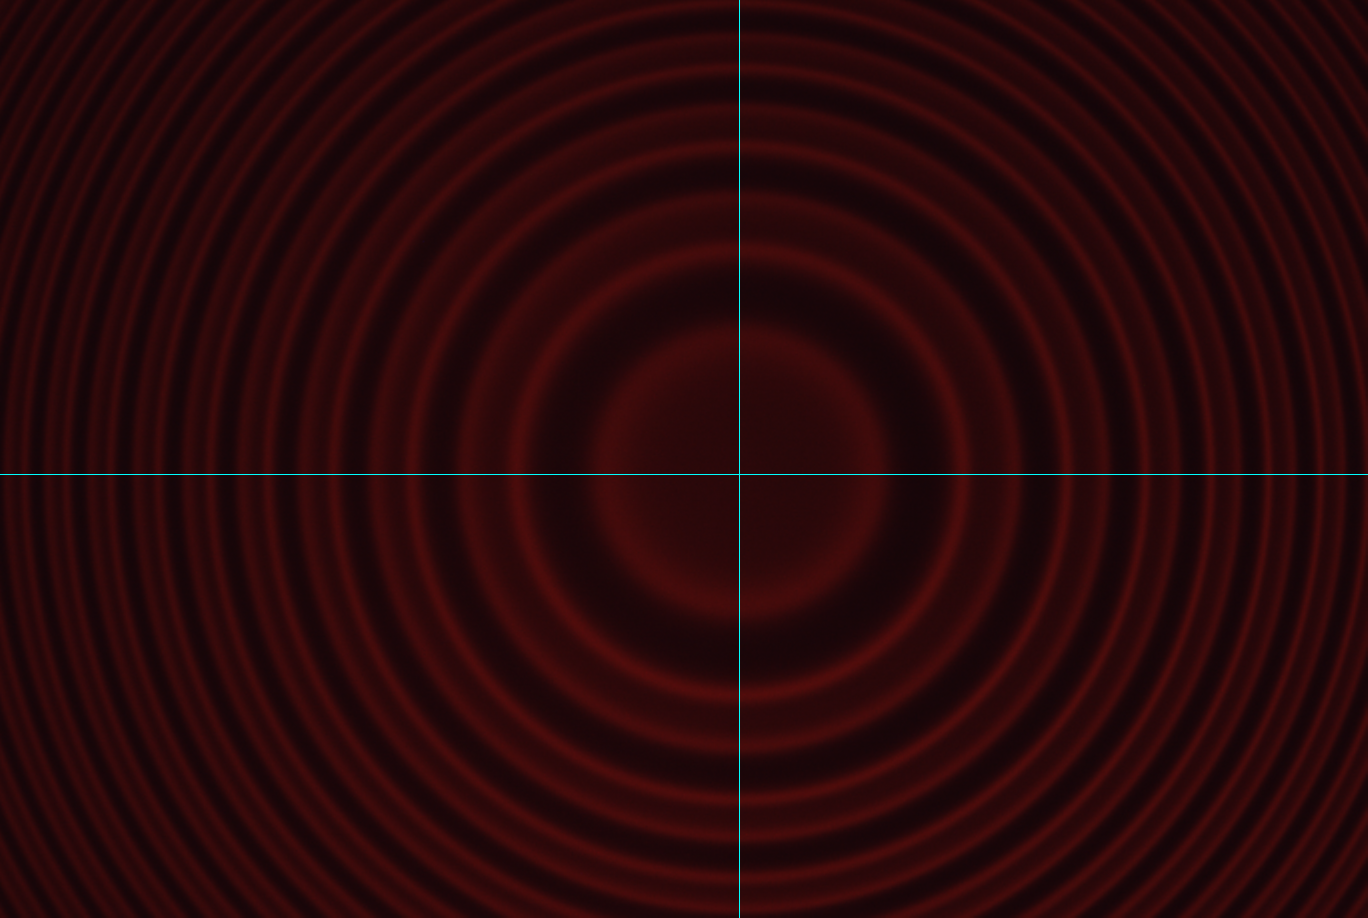
\includegraphics[width=.5\textwidth]{images/ZeemanFoto_003.png}}
    \subcaptionbox{Aufnahmen der Aufspaltung mit äußerem Magnetfeld ($\pi$-Komponente)}{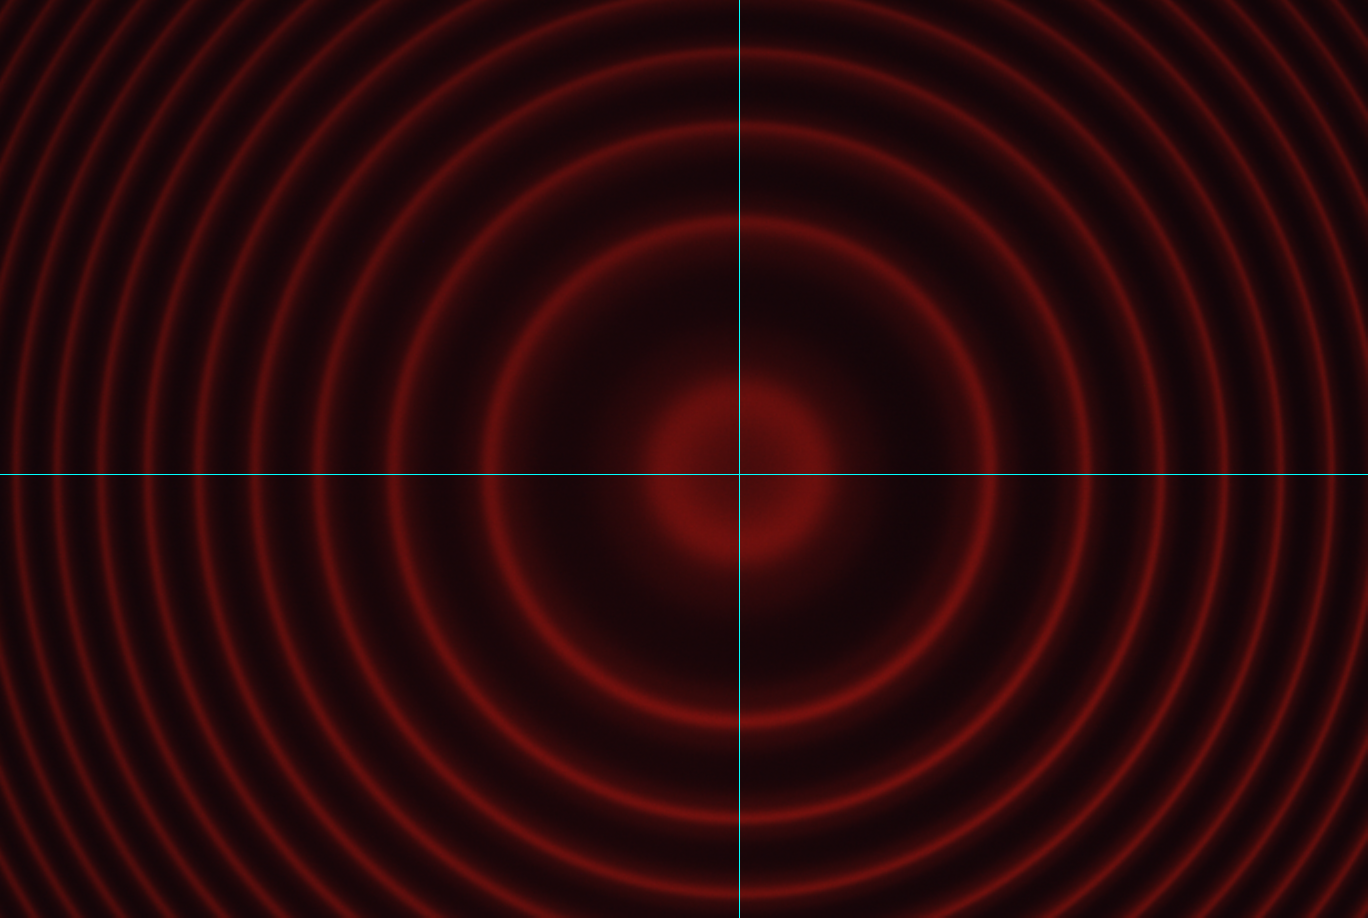
\includegraphics[width=.5\textwidth]{images/ZeemanFoto_004.png}}
    \caption{Aufnahmen in transversaler Konfiguration}
\end{figure}
\begin{figure}[!ht]
    \subcaptionbox{Aufnahmen der Aufspaltung ohne äußeres Magnetfeld}{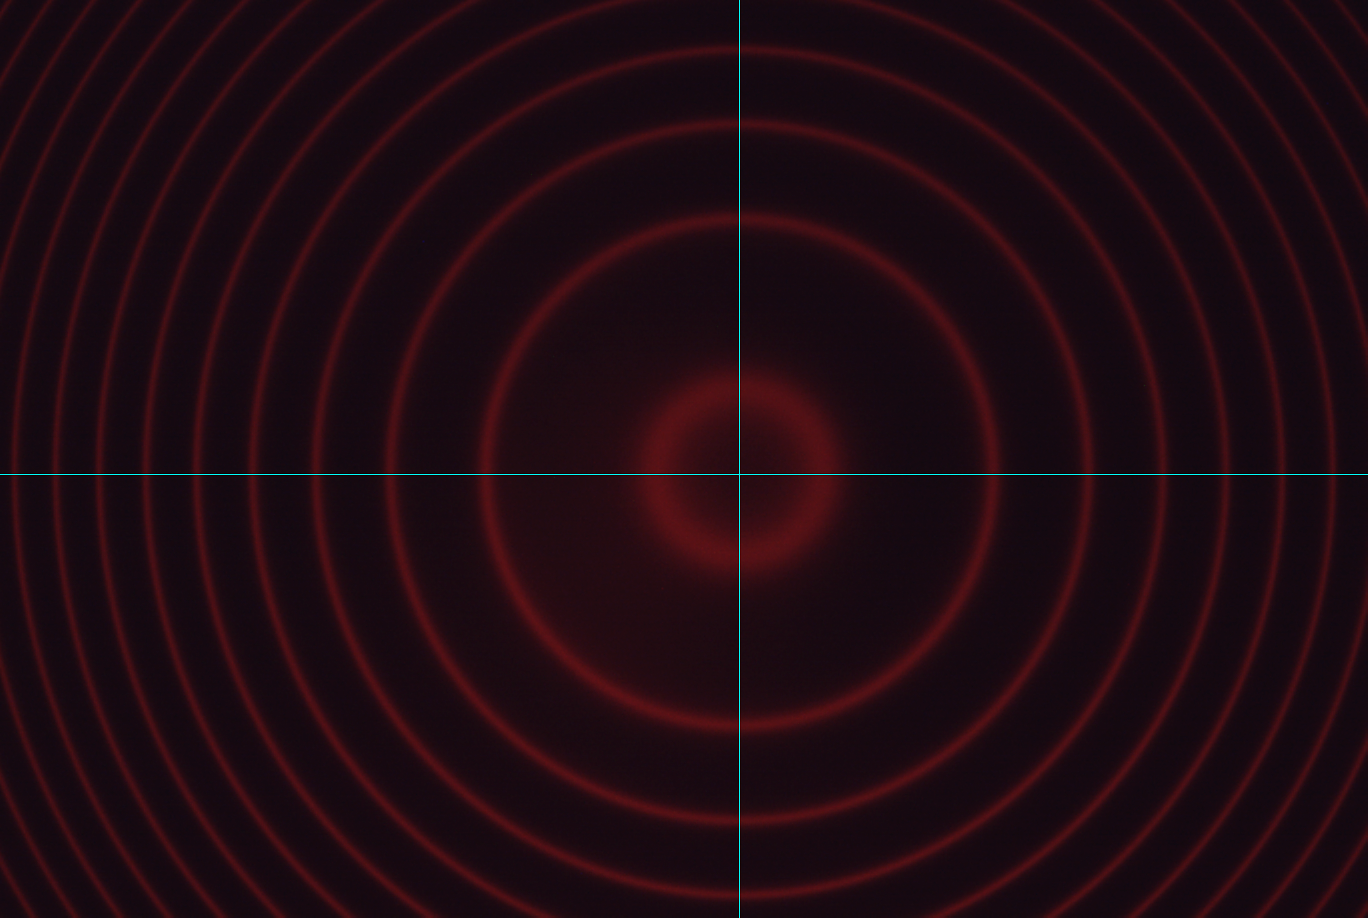
\includegraphics[width=.5\textwidth]{images/ZeemanFoto_008.png}}
    \subcaptionbox{Aufnahmen der Aufspaltung mit äußerem Magnetfeld}{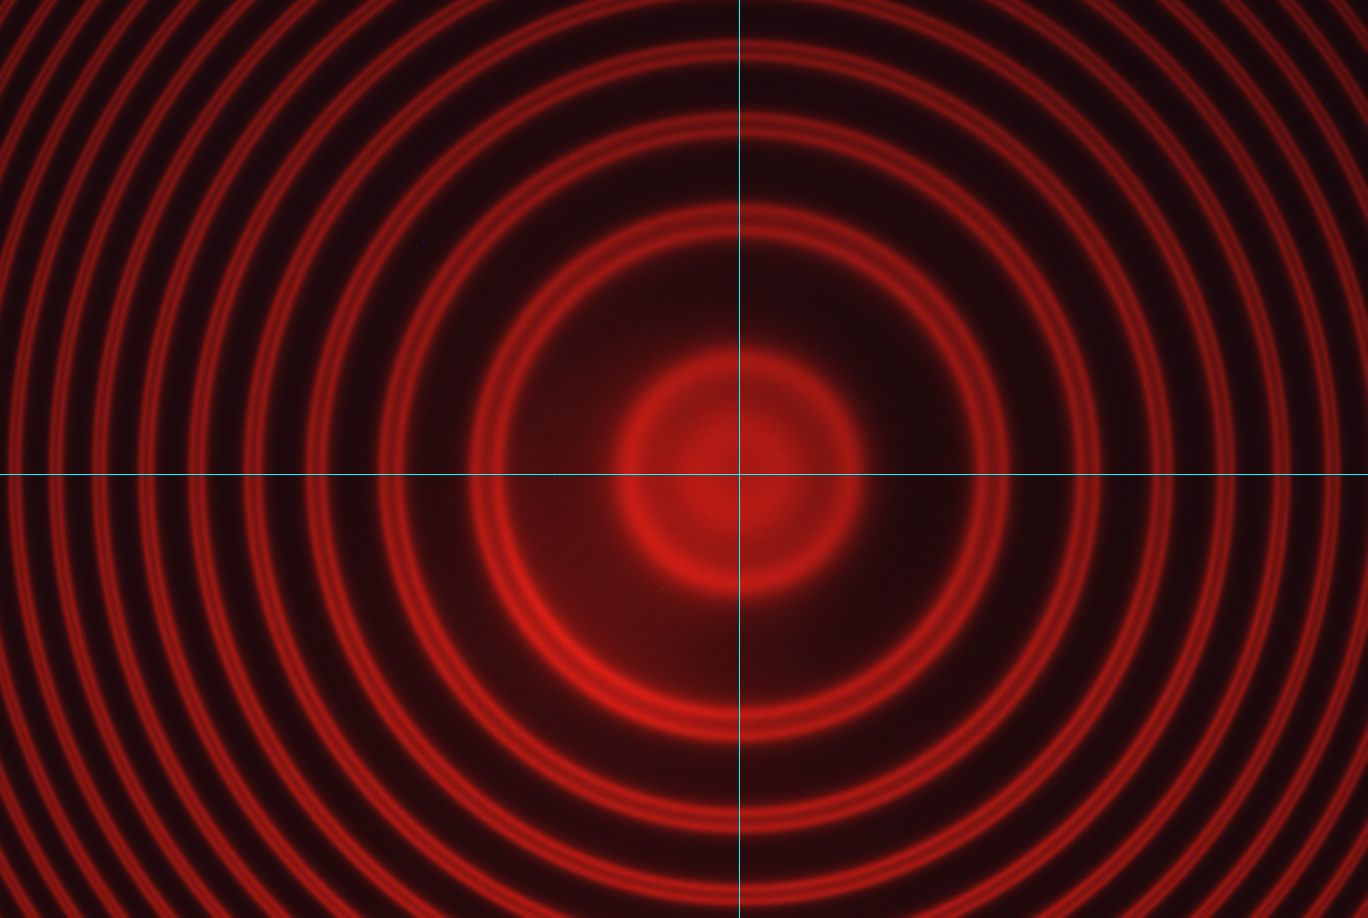
\includegraphics[width=.5\textwidth]{images/ZeemanFoto_009.png}}
    \subcaptionbox{Aufnahmen der Aufspaltung mit äußerem Magnetfeld ($\sigma^{+}$-Komponente)}{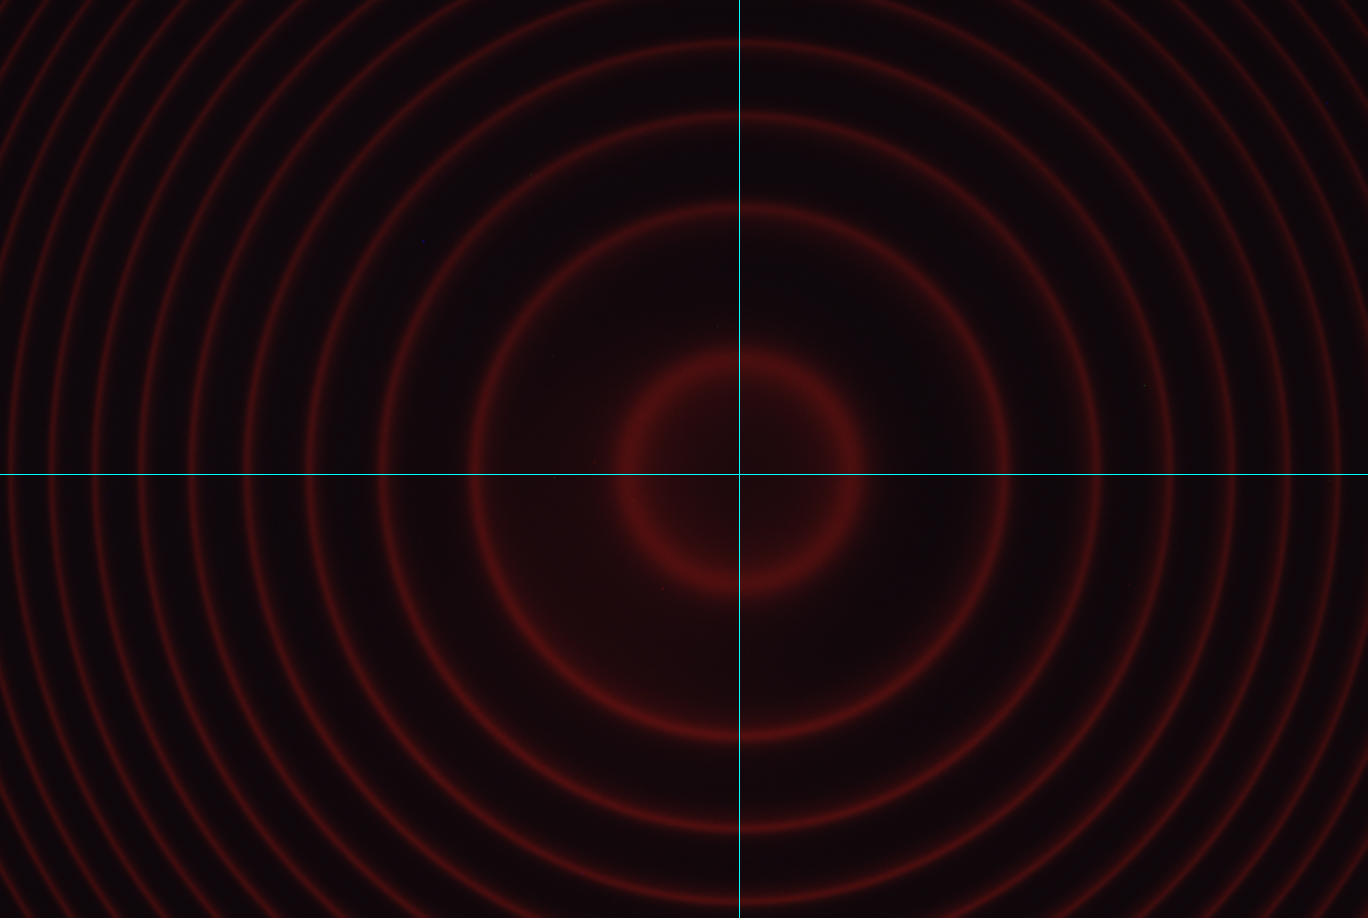
\includegraphics[width=.5\textwidth]{images/ZeemanFoto_010.png}}
    \subcaptionbox{Aufnahmen der Aufspaltung mit äußerem Magnetfeld ($\sigma^-$-Komponente)}{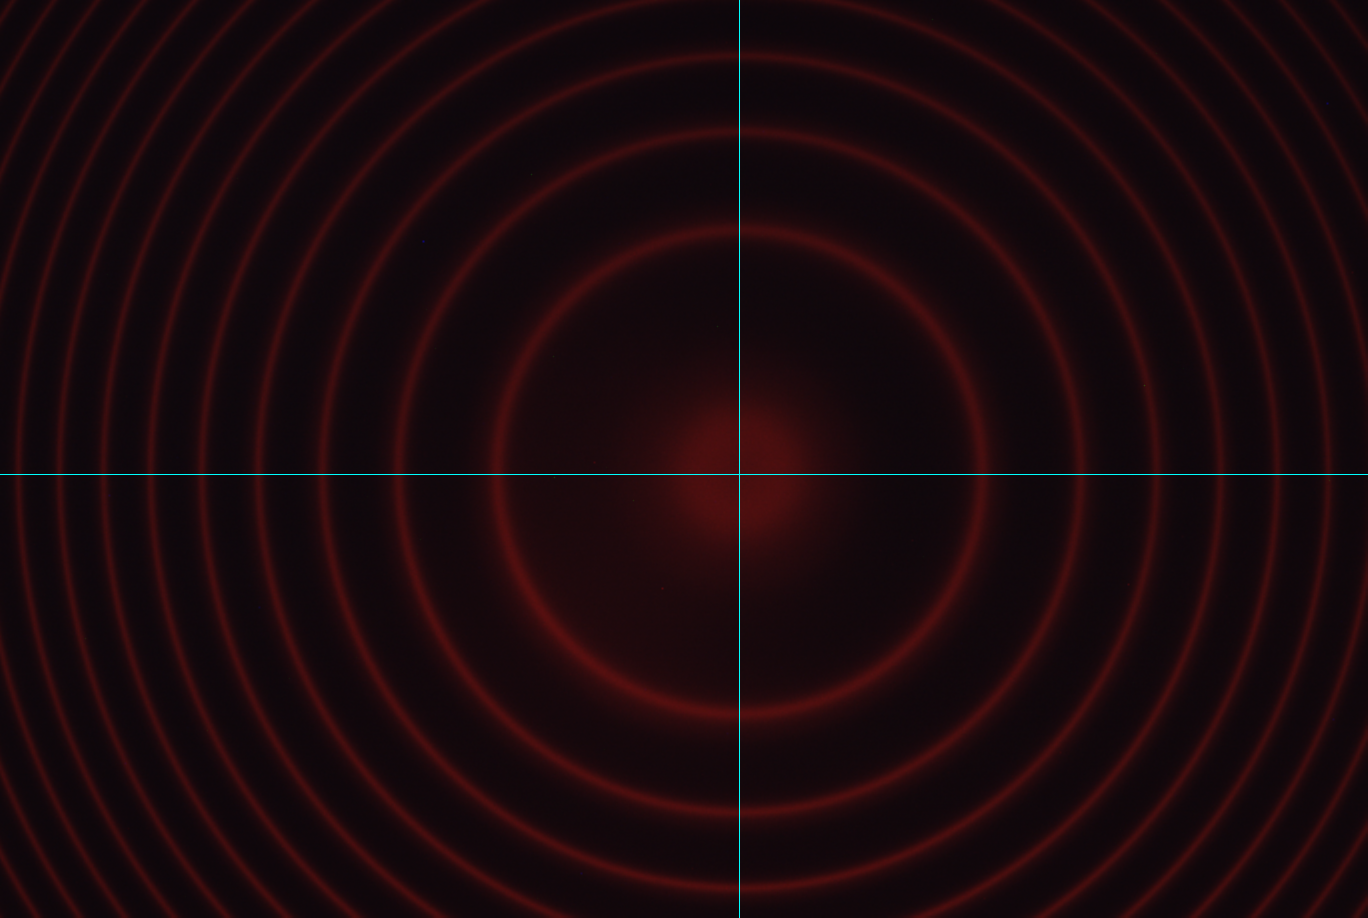
\includegraphics[width=.5\textwidth]{images/ZeemanFoto_011.png}}
    \caption{Aufnahmen in longitudinaler Konfiguration}
\end{figure}
\begin{figure}[!ht]
    \subcaptionbox{Anpassungskurve für $I = \SI{1}{\ampere}$}{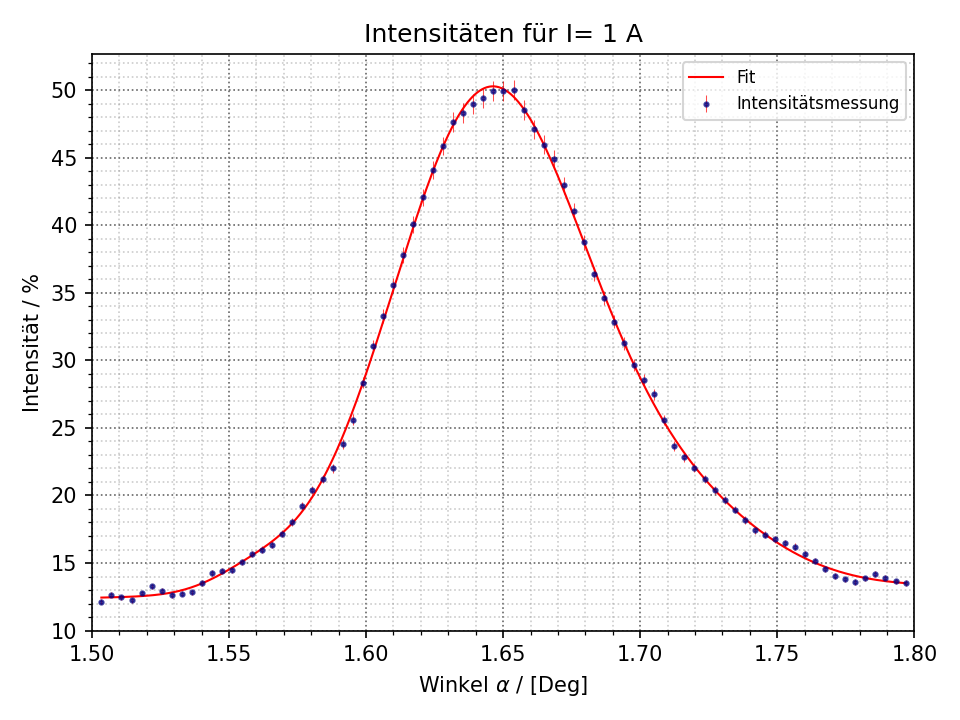
\includegraphics[width=.5\textwidth]{plots/peak_1A}}
    \subcaptionbox{Anpassungskurve für $I = \SI{2}{\ampere}$}{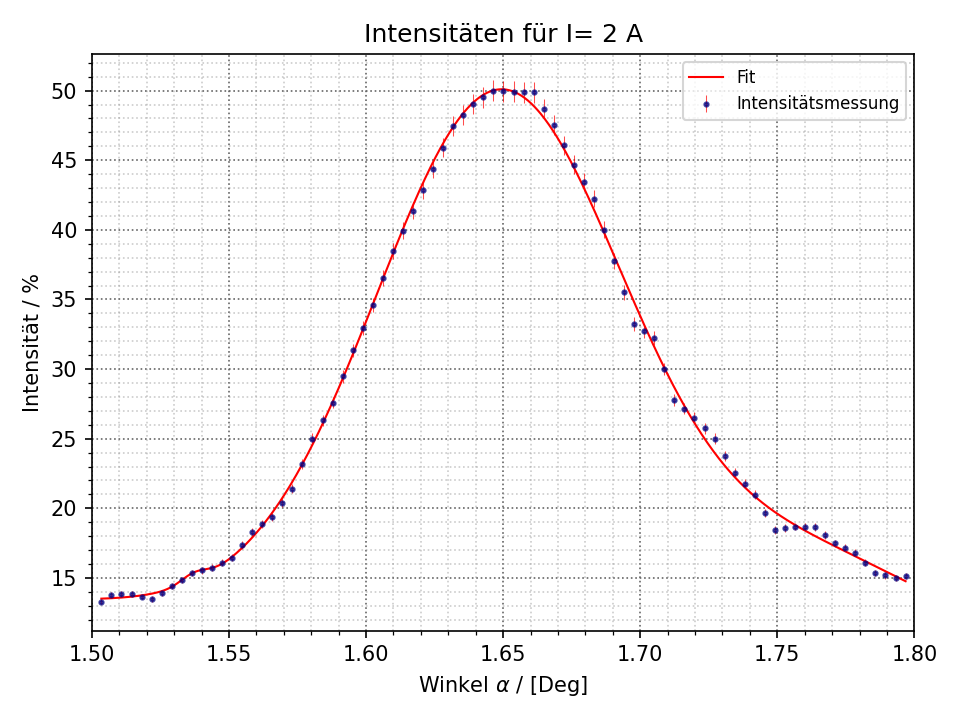
\includegraphics[width=.5\textwidth]{plots/peak_2A}}
    \subcaptionbox{Anpassungskurve für $I = \SI{3}{\ampere}$}{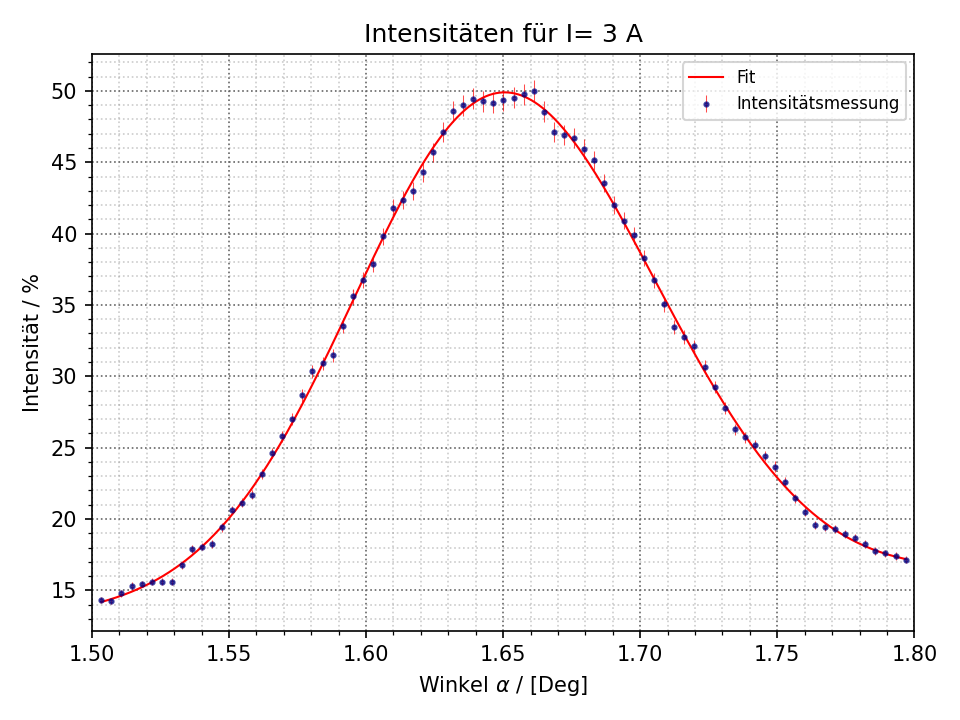
\includegraphics[width=.5\textwidth]{plots/peak_3A}}
    \subcaptionbox{Anpassungskurve für $I = \SI{4}{\ampere}$}{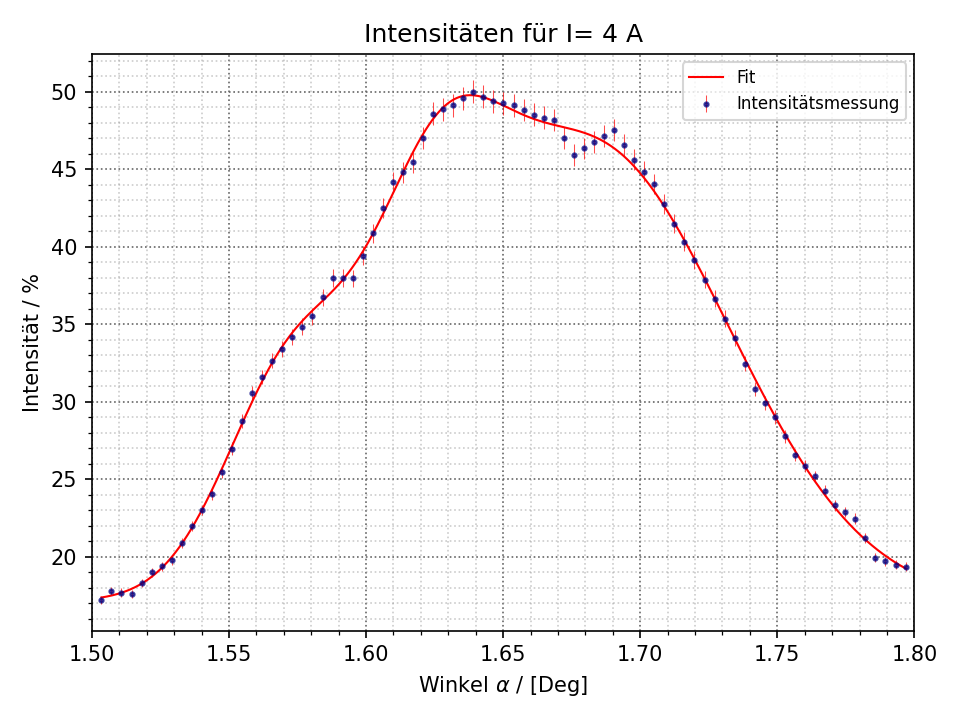
\includegraphics[width=.5\textwidth]{plots/peak_4A}}
    \subcaptionbox{Anpassungskurve für $I = \SI{5}{\ampere}$}{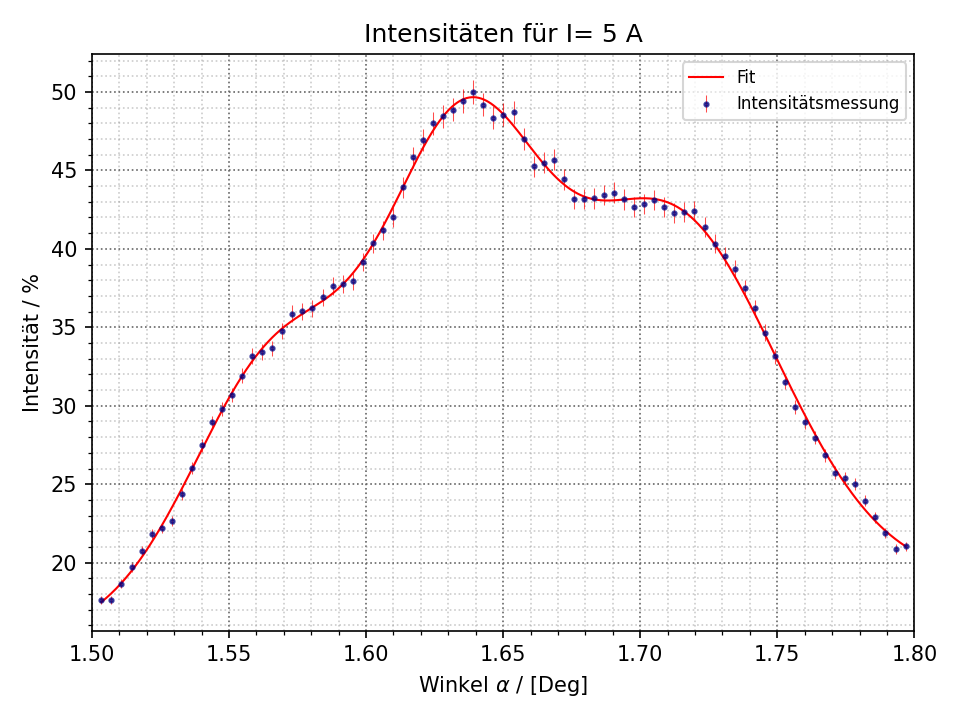
\includegraphics[width=.5\textwidth]{plots/peak_5A}}
    \subcaptionbox{Anpassungskurve für $I = \SI{6}{\ampere}$}{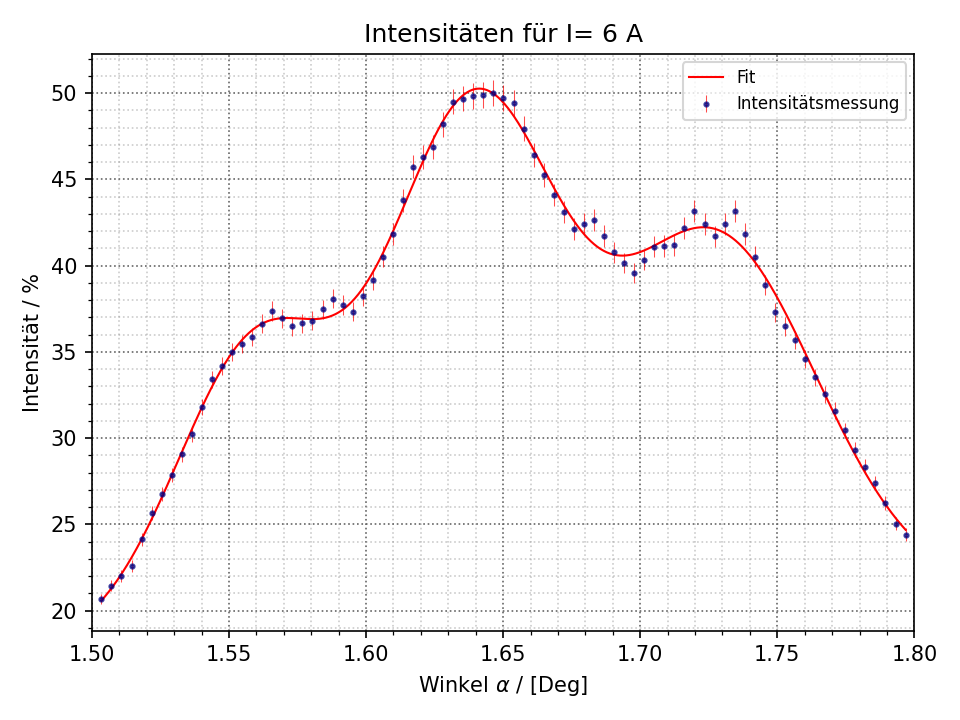
\includegraphics[width=.5\textwidth]{plots/peak_6A}}
    \caption{Mit der \texttt{CCD}-Kamera aufgenommene Intensitätsverläufe im Bereich \\$\alpha \in \left[\SI{1.5}{\degree}\; , \; \SI{1.8}{\degree}\right]$}\label{fig:peaks_all_a}
\end{figure}
\begin{figure}[!ht]
    \subcaptionbox{Anpassungskurve für $I = \SI{7}{\ampere}$}{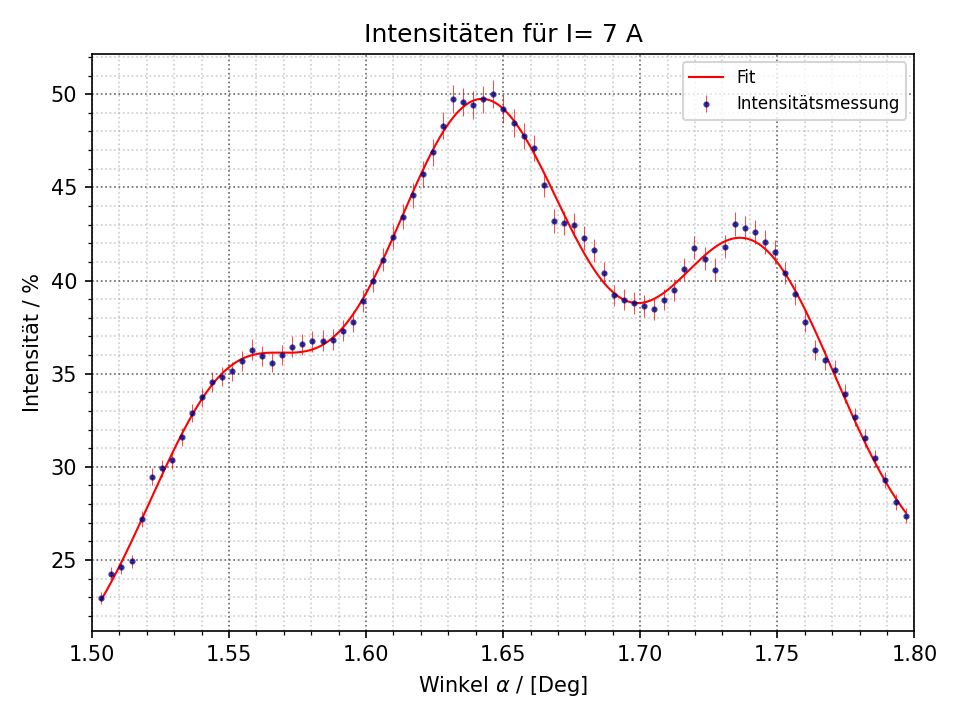
\includegraphics[width=.5\textwidth]{plots/peak_7A}}
    \subcaptionbox{Anpassungskurve für $I = \SI{8}{\ampere}$}{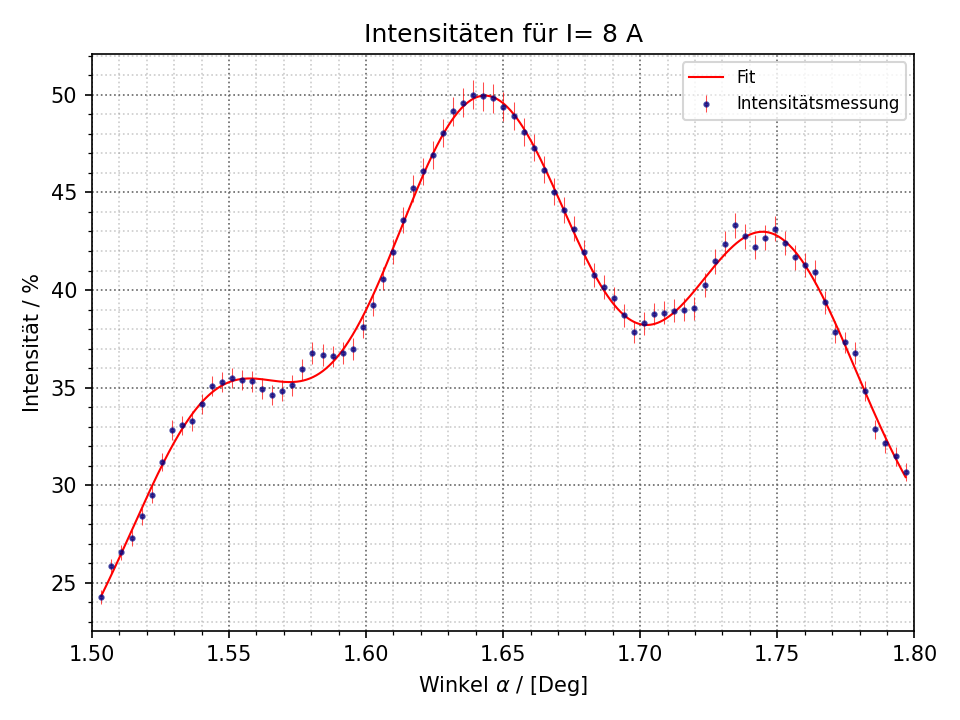
\includegraphics[width=.5\textwidth]{plots/peak_8A}}
    \subcaptionbox{Anpassungskurve für $I = \SI{9}{\ampere}$}{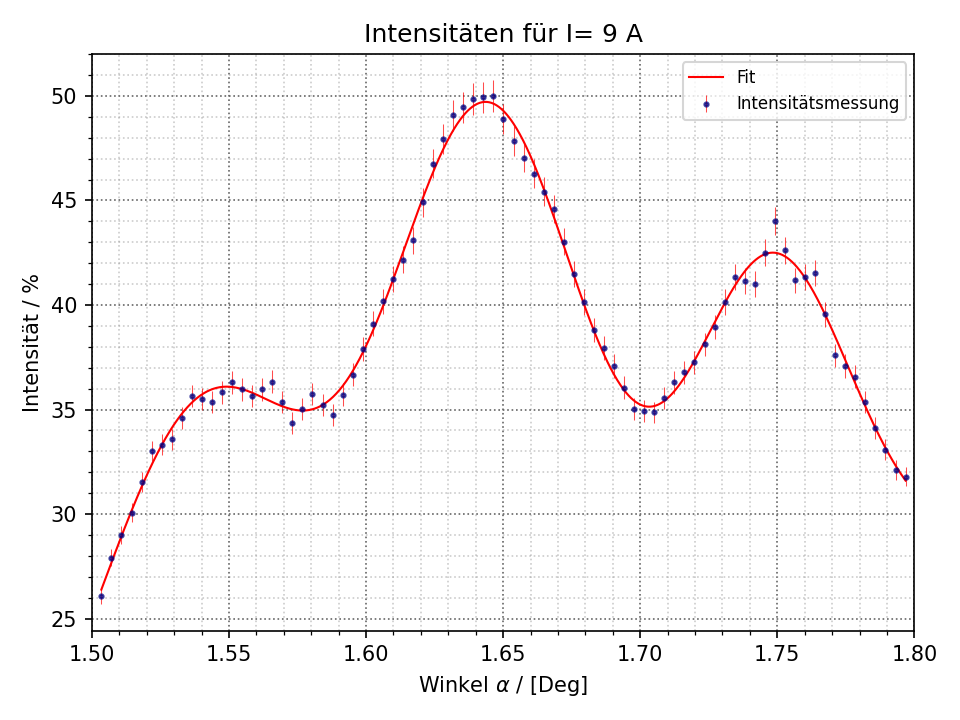
\includegraphics[width=.5\textwidth]{plots/peak_9A}}
    \subcaptionbox{Anpassungskurve für $I = \SI{10}{\ampere}$}{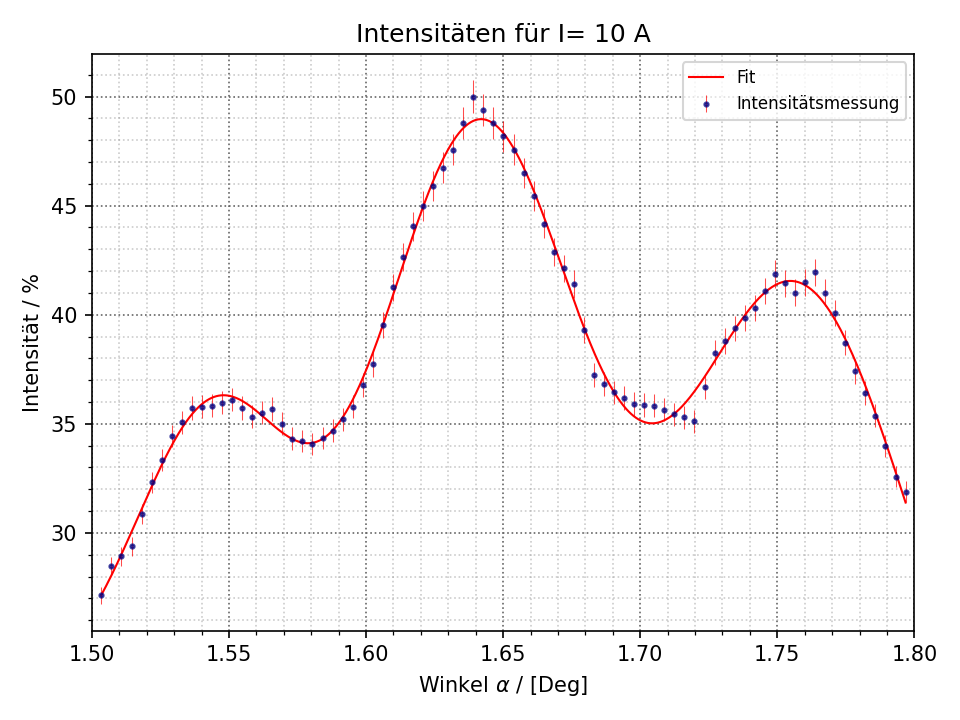
\includegraphics[width=.5\textwidth]{plots/peak_10A}}
    \caption{Mit der \texttt{CCD}-Kamera aufgenommene Intensitätsverläufe im Bereich \\$\alpha \in \left[\SI{1.5}{\degree}\; , \; \SI{1.8}{\degree}\right]$}\label{fig:peaks_all_b}
\end{figure}

%-----------------------------------------------------------------------
%-----------------------------------------------------------------------
%-----------------------------------------------------------------------
\clearpage
\subsection{Franck-Hertz}
\begin{figure}[!ht]
    \centering
    % first row: U1 & U2
    \subcaptionbox{$U_G$ = $\SI{2}{\volt}$ bei $\SI{165}{\celsius}$}{%
      \includegraphics[width=0.48\textwidth]{plots/UG2.png}%
    }
    \subcaptionbox{$U_G$ = $\SI{2.5}{\volt}$ bei $\SI{165}{\celsius}$}{%
      \includegraphics[width=0.48\textwidth]{plots/UG2_5.png}%
    }
  
    \medskip
    % second row: U3 & U4
    \subcaptionbox{$U_G$ = $\SI{3}{\volt}$ bei $\SI{165}{\celsius}$}{%
      \includegraphics[width=0.48\textwidth]{plots/UG3.png}%
    }
    \subcaptionbox{$U_G$ = $\SI{3.5}{\volt}$ bei $\SI{165}{\celsius}$}{%
      \includegraphics[width=0.48\textwidth]{plots/UG3_5.png}%
    }
  
    \medskip
    % third row: U5 & U6
    \subcaptionbox{$U_G$ = $\SI{4}{\volt}$ bei $\SI{165}{\celsius}$}{%
      \includegraphics[width=0.48\textwidth]{plots/UG4.png}%
    }

  \caption{Anodenspannungskurven in Abhängigkeit der Gegenspannung bei konstanter Temperatur von $T$ = $\SI{165}{\celsius}$.}
\label{fig:UGall}
\end{figure}

\begin{figure}[!ht]
    \centering
    % first row: U1 & U2
    \subcaptionbox{$T$ = $\SI{165}{\celsius}$ bei $\SI{3}{\volt}$  }{%
      \includegraphics[width=0.48\textwidth]{plots/T165.png}%
    }
    \subcaptionbox{$T$ = $\SI{170}{\celsius}$ bei $\SI{3}{\volt}$}{%
      \includegraphics[width=0.48\textwidth]{plots/T170.png}%
    }
  
    \medskip
    % second row: U3 & U4
    \subcaptionbox{$T$ = $\SI{175}{\celsius}$ bei $\SI{3}{\volt}$}{%
      \includegraphics[width=0.48\textwidth]{plots/T175.png}%
    }
    \subcaptionbox{$T$ = $\SI{180}{\celsius}$ bei $\SI{3}{\volt}$ }{%
      \includegraphics[width=0.48\textwidth]{plots/T180.png}%
    }

  \caption{Anodenspannungskurven in Abhängigkeit der Temperatur bei konstanter Gegenspannung von $U_G$ = $\SI{3}{\volt}$.}
\label{fig:Tall}
\end{figure}


\clearpage
\section{Tabellen}
\subsection{Zeemann-Effekt}
\begin{table}[ht]
    \centering
    \footnotesize
    \begin{tabular}{c *{5}{c}}
        \toprule
        Parameter & {1} & {2} & {3} & {4} & {5} \\
        \midrule
        $\chi_\text{red}^2$ & 1.34      & 1.68              & 1.11          & 0.72              & 0.83 \\
        $a$         & 2.85 (0.92)       & -8.53 (9.96)      & 9.92 (---)    & 0.043 (1.26)      & 10.96 (2.10) \\
        $b$         & 8.15 (1.43)       & 26.12 (15.02)     & -1.57 (---)   & 17.05 (1.94)      & -0.96 (3.53) \\
        $A_1$       & 0.046 (0.015)     & 0.008 (0.0043)    & 7.1e-7 (---)  & 0.803 (0.077)     & 1.336 (0.185) \\
        $\sigma_1$  & 0.015 (0.0030)    & 0.0049 (0.0025)   & 0.045 (---)   & 0.024 (0.0013)    & 0.031 (0.0024) \\
        $\mu_1$     & 1.559 (0.0029)    & 1.537 (0.0022)    & 1.547 (---)   & 1.573 (0.0022)    & 1.569 (0.0030) \\
        $A_2$       & 3.201 (0.228)     & 4.301 (0.194)     & 4.672 (---)   & 0.831 (0.191)     & 1.835 (0.228) \\
        $\mu_2$     & 1.644 (0.0023)    & 1.649 (0.0009)    & 1.649 (---)   & 1.625 (0.0018)    & 1.635 (0.0014) \\
        $\sigma_2$  & 0.0349 (0.0012)   & 0.0453 (0.0008)   & 0.0533 (---)  & 0.0229 (0.0021)   & 0.0279 (0.0017) \\
        $A_3$       & 0.488 (0.243)     & 0.575 (0.376)     & 0.146 (---)   & 3.705 (0.235)     & 2.473 (0.194) \\
        $\mu_3$     & 1.711 (0.013)     & 1.761 (0.0087)    & 1.725 (---)   & 1.682 (0.0027)    & 1.709 (0.0022) \\
        $\sigma_3$  & 0.0340 (0.0062)   & 0.0426 (0.0100)   & 0.0346 (---)  & 0.0502 (0.0020)   & 0.0403 (0.0020) \\
        \bottomrule
    \end{tabular}
    \vspace{1em}
    \begin{tabular}{c *{5}{c}}
        \toprule
        Parameter & {6} & {7} & {8} & {9} & {10} \\
        \midrule
        $\chi_\text{red}^2$ & 0.858 & 0.825 & 0.620 & 0.674 & 0.669 \\
        $a$         & 10.04 (3.07)      & 18.77 (4.66)      & 22.47 (6.25)      & 46.72 (13.07)     & -21.55 (15.45) \\
        $b$         & 2.92 (4.93)       & -10.10 (8.08)     & -15.89 (10.80)    & -56.16 (23.80)    & 54.46 (22.96) \\
        $A_1$       & 1.223 (0.128)     & 1.183 (0.195)     & 1.226 (0.234)     & 1.896 (0.566)     & 1.029 (0.194) \\
        $\sigma_1$  & 0.0293 (0.0017)   & 0.0312 (0.0025)   & 0.0325 (0.0027)   & 0.0387 (0.0043)   & 0.0288 (0.0022) \\
        $\mu_1$     & 1.560 (0.0015)    & 1.551 (0.0014)    & 1.546 (0.0012)    & 1.541 (0.0019)    & 1.545 (0.0010) \\
        $A_2$       & 2.263 (0.117)     & 2.608 (0.0833)    & 2.692 (0.105)     & 2.509 (0.207)     & 2.673 (0.259) \\
        $\mu_2$     & 1.639 (0.00087)   & 1.641 (0.00074)   & 1.642 (0.00057)   & 1.643 (0.00091)   & 1.642 (0.00051) \\
        $\sigma_2$  & 0.0311 (0.0014)   & 0.0364 (0.0014)   & 0.0375 (0.0010)   & 0.0351 (0.0007)   & 0.0363 (0.0008) \\
        $A_3$       & 2.010 (0.188)     & 1.542 (0.155)     & 1.578 (0.189)     & 1.202 (0.151)     & 2.541 (0.716) \\
        $\mu_3$     & 1.727 (0.0015)    & 1.739 (0.0010)    & 1.746 (0.00086)   & 1.747 (0.00078)   & 1.758 (0.0018) \\
        $\sigma_3$  & 0.0375 (0.0021)   & 0.0325 (0.0017)   & 0.0331 (0.0018)   & 0.0288 (0.0015)   & 0.0410 (0.0042) \\
        \bottomrule
    \end{tabular}
    \caption[Anpassungsparameter zur Messreihe \textsc{Zeeman}-Effekt]{Anpassungsparameter der Gaußkurven aus der Messreihe zum \textsc{Zeeman}-Effekt. Die dazugehörigen Abbildungen sind \crefrange{fig:peaks_all_a}{fig:peaks_all_b} zu finden.}\label{tab:langzeeman-fit}
\end{table}
\normalsize
%-----------------------------------------------------------------------
%-----------------------------------------------------------------------
%-----------------------------------------------------------------------
\clearpage
\subsection{Franck-Hertz}
\begin{table}[h!]
    \centering
    \sisetup{uncertainty-mode=separate}
    \begin{tabular}{
      l|
      S[table-format=1.3(3)]
      S[table-format=1.3(3)]
    }
    \toprule
    \multicolumn{1}{c|}{$U_G$ [V] (bei Temperatur = $\SI{165}{\degreeCelsius}$)} &
    \multicolumn{1}{c}{$\Delta E$ [eV]} &
    \multicolumn{1}{c}{$\sigma$ [V]} \\
    \midrule
    2.0 & 4.830 \pm 0.183 & 0.817 \pm 0.328 \\
    2.5 & 4.810 \pm 0.220 & 0.921 \pm 0.107 \\
    3.0 & 4.830 \pm 0.320 & 0.903 \pm 0.085 \\
    3.5 & 4.840 \pm 0.260 & 0.862 \pm 0.082 \\
    4.0 & 4.850 \pm 0.207 & 0.635 \pm 0.300 \\
    \bottomrule
    \end{tabular}
    \caption{Gemittelte $\Delta E$ und Breite der angepassten Gaußkurven für jede Gegenspannung}
  \label{tab:franckU2}
  \end{table}
  \vspace{1em}
  \begin{table}[h!]
    \centering
    \sisetup{uncertainty-mode=separate}
    \begin{tabular}{
      l|
      S[table-format=1.3(3)]
      S[table-format=1.3(3)]
    }
    \toprule
    \multicolumn{1}{c|}{Temperatur [\si{\degreeCelsius}] (bei $U_G$ = $3 \si{\volt}$)} &
    \multicolumn{1}{c}{$\Delta E$ [eV]} &
    \multicolumn{1}{c}{$\sigma$ [V]} \\
    \midrule
    165 & 4.840 \pm 0.193 & 0.911 \pm 0.074 \\
    170 & 4.830 \pm 0.183 & 0.917 \pm 0.065 \\
    175 & 4.800 \pm 0.158 & 0.927 \pm 0.061 \\
    180 & 4.810 \pm 0.037 & 0.900 \pm 0.080 \\
    \bottomrule
    \end{tabular}
    \caption{Gemittelte $\Delta E$ und Breite der angepassten Gaußkurven für jede Temperatur}
  \label{tab:franckT}
  \end{table}
  
\clearpage
\section{Github-Repository}
Link zum Github-Repository: \url{https://github.com/itzhaQQ/P4.git}
